% !TeX root = ../main.tex

\chapter{Platform Design}\label{chapter:platform-design}

The platform was designed to isolate the aerodynamic effects of fixed lifting surfaces on a quadrotor without introducing new actuators or changing the control structure. The result is an X-wing configuration in which each rotor arm forms a fixed lifting surface. The design goal was to achieve measurable lift at moderate forward speeds (5--15\,\si{\meter\per\second}) while preserving the agility and controllability of a conventional multirotor.

\section{Configuration and Layout}

The vehicle retains the standard X-shaped quadrotor geometry but extends each arm into a symmetric wing section, producing a cross-shaped planform. This geometry satisfies three constraints:

\begin{itemize}
  \item \textbf{Dynamic symmetry}: Equal inertias and aerodynamic properties in roll and pitch enable identical control gains across both axes.
  
  \item \textbf{Passive lift generation}: Each wing contributes lift proportional to its forward velocity component without interfering with rotor control authority.
  
  \item \textbf{Mechanical simplicity}: No additional servos or morphing structures are introduced; all aerodynamic effects are passive.
\end{itemize}

The $\pm 45^{\circ}$ alternating dihedral and anhedral angles maintain directional symmetry, ensuring that any heading can serve as ``forward'' flight. Although such extreme dihedral is aerodynamically suboptimal compared with planar wings, it simplifies the control problem by avoiding preferred directions and limiting coupling between roll and pitch.

The wings employ a NACA~0015 symmetric profile with 0.25\,m chord and 0.45\,m span, yielding an aspect ratio of $\approx 1.8$. These dimensions were selected to ensure that at $\approx 10$--12\,\si{\meter\per\second} the predicted lift equals or slightly exceeds the vehicle weight, based on first-order thin-airfoil theory. The design therefore enables significant lift without requiring impractically large structures.

\section{Structural Design and Manufacturing}

Each wing consists of a 3D-printed aerodynamic shell reinforced by two 10\,mm carbon spars. The hybrid construction provides sufficient bending stiffness while keeping individual wing mass below 180\,g. Structural resonance tests indicated the first bending mode well above the control bandwidth, confirming negligible coupling to attitude dynamics.

The central frame clamps the eight spars from the four wings and houses all electronics. Motors are mounted on integrated endcaps that also serve as landing feet, providing $5^{\circ}$ outward motor tilt for yaw authority. The total diagonal motor-to-motor distance is 1.1\,m, yielding a compact yet aerodynamically relevant planform.

\begin{figure}[htbp]
\centering
\includegraphics[width=0.48\linewidth]{figures/wing_transparent.png}
\hfill
\includegraphics[width=0.48\linewidth]{figures/wing_sliced.png}
\caption{Wing structure showing the hollow internal geometry with channels for carbon fiber spars (left) and printed aerodynamic shell (right). Each wing weighs approximately 176\,g including carbon reinforcement.}
\label{fig:wing_structure}
\end{figure}

\begin{figure}[htbp]
\centering
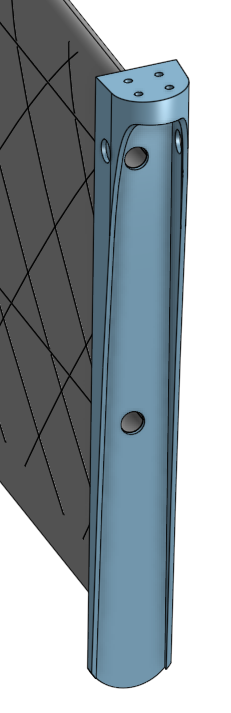
\includegraphics[height=0.4\linewidth]{figures/foot.png}
\caption{Wing endcap component serving as motor mount and landing foot. This multi-functional part positions the motor ahead of the leading edge with $\pm 5^{\circ}$ tilt for yaw control and extends downward to protect the wing trailing edge during landing.}
\label{fig:wing_foot}
\end{figure}

\begin{figure}[htbp]
\centering
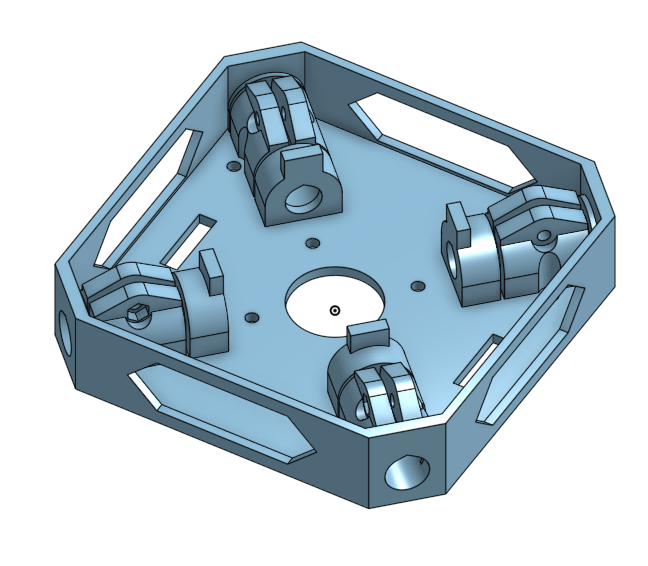
\includegraphics[width=0.6\linewidth]{figures/core.png}
\caption{Central core structure that clamps the carbon fiber spars. Two identical cores are used: one houses the ESC, flight controller, and batteries (top), while the other serves as a structural clamp for the lower spars (bottom).}
\label{fig:core_structure}
\end{figure}

\section{Aerodynamic Estimates}

At 12\,\si{\meter\per\second}, using $\rho = 1.225$\,kg\,m$^{-3}$, $S = 0.318$\,m$^{2}$, $C_L = 0.97$, $C_D = 0.025$, the theoretical lift and drag are:
\[
L \approx 27.2\,\text{N}, \quad D \approx 0.7\,\text{N}.
\]
This corresponds to $\approx 110\,\%$ of the vehicle's 2.5\,kg weight, suggesting that in steady forward flight the rotors primarily counteract drag and provide control authority. Although these values are first-order estimates and neglect prop-wash interaction, they provide a reference for disturbance magnitudes that the INDI controller must compensate.

More accurate modeling would require CFD or wind-tunnel validation; however, for the scope of this study the analytical approximation suffices to show that aerodynamic lift is on the same order as vehicle weight and therefore cannot be ignored in flight analysis, even if it remains unmodeled in control.

A detailed comparison of the NACA~0015 baseline airfoil against an improved AG25 airfoil, including aerodynamic performance metrics and their correlation with flight test results, is presented in Chapter~\ref{chapter:experiments-evaluation}.

\section{Propulsion and Actuation}

The propulsion system uses T-MOTOR VELOX V2808 motors with HQProp 7$\times$3.5$\times$3 propellers, producing up to 22\,N static thrust per motor. The total thrust-to-weight ratio exceeds 3, allowing aggressive maneuvers and ensuring that aerodynamic loads never saturate actuator authority.

Motors are tilted outward by $5^{\circ}$ to enhance yaw torque. The corresponding geometry is embedded in the allocation matrix used by the controller; no additional coupling compensation is required. Static thrust characterization (Chapter~\ref{chapter:experiments-evaluation}, Section~\ref{sec:thrust-identification}) confirms a quadratic thrust--RPM relation with $R^2 = 0.997$, validating consistency between analytical assumptions and measured performance.

The complete airframe mass, including avionics and batteries, is $\approx 2.5$\,kg. The center of gravity lies at the geometric center, aligned with the intersection of the four wing roots, minimizing trim moments during hover.

\section{Summary}

The X-wing configuration provides a mechanically simple and dynamically symmetric platform in which aerodynamic forces are large enough to challenge the controller but not strong enough to destabilize the system. The design therefore fulfills the thesis objective: to expose an INDI-controlled quadrotor to significant unmodeled aerodynamic effects without introducing additional actuation or transition mechanisms.

A second airframe variant was later developed to improve aerodynamic efficiency in forward flight.
This refined configuration reduced the dihedral from $\pm 45^{\circ}$ to $\pm 20^{\circ}$ and replaced the NACA~0015 airfoil with an AG25 profile.
The lower dihedral reduces projected area loss and induced drag, while the AG25's cambered geometry increases lift-to-drag ratio at typical cruise Reynolds numbers.
The aerodynamic coefficient and agility analyses in Chapter~\ref{chapter:experiments-evaluation} include both configurations, while the outdoor power-efficiency validation employs the refined AG25 design to quantify the performance of the final, optimized prototype.